% !TeX root = Body.tex

\chapter{Analysis based on Stochastic Matrices}
\label{chap:ProofEx}

In this chapter, we prove the existence of the non-equilibrium stationary state in our model with a half sliding for arbitrary velocities $v>0$. In the first section, we discuss the formulation by stochastic matrices, and then see Monte Carlo simulations and the stochastic matrices are equivalent in terms of the probability with a simple example. In the following two sections, we prove several facts for stochastic matrices, which ensures that almost all Monte Carlo simulations converge to a equilibrium state and its uniqueness, and then the properties are taken over and lead to a unique stationary state even if the matrix contains a kind of perturbation factors. In the last two sections, we propose the way to construct the matrix for both equilibrium cases and non-equilibrium stationary cases, and discuss the distributions of their eigenvalues in terms of the convergence.

\section{A Simple Example: Stochastic Ising Model with $N$-spins}
Monte Carlo simulations for lattice spin systems extract the relevant subspace from the full space instead of an exact calculation of the partition function using a stochastic process. The subspace depends on given parameters and if we use the canonical distribution with a fixed temperature $T$, the temperature determines the subspace. The stochastic process is expressed as a trajectory of variables by the time in the subspace. Averaging the trajectory for an enough long time, we can compute physical quantities with any desired accuracy.

We now consider a matrix form of the stochastic process. For example, the one-dimensional Ising chain with $N$-spins has $2^{N}$ states. If we labeled each of the states by $i=1,2,\dots,2^{N}$, we can write the stochastic time evolution of the system by a set of the existence probabilities $\{p_{i}(t)\}$ such that the system is in the $i$-th state at a time $t$, and the transition probabilities $T_{ij}$ such that the system in the $j$-th state changes to the $i$-th state. Note that not the transition probabilities $T_{ij}$ but the existence probabilities $\{p_{i}(t)\}$ play the role of time evolution.

We additionally define the conditional probability $\tilde{p}_{ij}(t)$ such that the system in the $j$-th state at a time $t$ changes to the $i$-th state at the next time $t+1$. Using the conditional probability, we can derive the relation between the existence probability $p_{i}(t)$ and the transition probability $T_{ij}$ as
\begin{align}
\tilde{p}_{ij}(t + 1) = T_{ij} p_{j}(t)\quad\text{for $1\leq i,j\leq 2^{N}$}.
\end{align}
From a property as the probability, it should hold that $\sum_{i=1}^{2^{N}}p_{i}(t)=1$ and $p_{i}(t) \ge 0$ ($i=1,2,\dots,2^{N}, t\in\mathbb{R}$). The conditional probability $\tilde{p}_{ij}(t)$ should also satisfy the condition that $\sum_{j=1}^{2^{N}}\tilde{p}_{ij}(t) = p_{i}(t+1)$ ($i=1,2,\dots,2^{N}, t\in\mathbb{R}$). Then we have
\begin{align}
p_{i}(t+1) = \sum_{j=1}^{2^{N}}\tilde{p}_{ij}(t + 1) = \sum_{j=1}^{2^{N}}T_{ij}p_{j}(t)\quad\text{for $1\leq i\leq 2^{N}$, $t\in\mathbb{R}$}.
\end{align}
In the other words, the system can be described by the probability vector $\bm{p}(t):={}^{\rm t}\left(p_{1}(t),p_{2}(t),\dots,p_{2^{N}}(t)\right)$ and the stochastic matrix $\hat{T}:=\left(T_{ij}\right)$ as
\begin{align}
\bm{p}(t + 1) = \hat{T}\bm{p}(t)\quad\text{for $t\in\mathbb{R}$}.
\end{align}
In Monte Carlo simulations, we often trace the trajectory of a component of the vector $\bm{p}(t)$, thus we rarely need to construct the matrix $\hat{T}$. But it is helpful for us to consider such the matrix when we discuss the convergence to the stationary state or its uniqueness. These discussions are valid for general $\Omega$-dimensional state spaces, thus we denote the number of states by $\Omega$ from now on.

\section{General Theory of Stochastic Matrices}

In this section we discuss the conditions which ensure a convergence of the corresponding Monte Carlo simulation to a unique stationary state. We first define the stochastic matrix and discuss fundamental properties of the stochastic matrix. We next discuss the properties which result from an additional condition called \textit{weak/strong connectivity}, which leads the existence and the uniqueness of a stationary state. We also see that we can construct a stochastic matrix which leads to any desired stationary state under the so-called \textit{detailed balanced condition}.

From the condition $\sum_{i=1}^{\Omega}p_{i}(t)=1$ and $p_{i}(t) \ge 0$ ($i=1,2,\dots,\Omega, t\in\mathbb{R}$), we have a set of properties $\sum_{i=1}^{\Omega}T_{ij} = 1$, $T_{ij}\ge 0$ ($1\leq i\leq \Omega$). Any matrix with these conditions is called \textit{stochastic matrix} and shows the following interesting property:
\begin{theorem}
	Let $\hat{T}$ be a stochastic matrix, then all absolute values of eigenvalue are less than or equal to $1$. For any eigenvector $\bm{x}={}^{\rm t}\{x_{1},x_{2},\dots,x_{\Omega}\}$ which does \textit{not} belong to the eigenvalue $1$, it additionally holds that
	\begin{align}
	\sum_{i=1}^{\Omega}x_{j}=0.
	\end{align}
\end{theorem}
We now define the vector $\bm{d}:={}^{\rm t}\left(1,1,\dots,1\right)$ to prove all facts after this.
\begin{proof}
	For any stochastic matrix $\hat{T}$, we have
	\begin{align}
	&\left({}^{\rm t}\hat{T}\bm{d}\right)_{i}=\sum_{j=1}^{\Omega}\left({}^{t}T\right)_{ij}d_{j}=\sum_{j=1}^{\Omega}T_{ji}d_{j}=\sum_{j=1}^{\Omega}T_{ji}=1\quad\text{for $i=1,2,\dots,\Omega$},\\
	\Longleftrightarrow\quad &{}^{\rm t}\hat{T}\bm{d} = \bm{d}.
	\end{align}
	Therefore the matrix ${}^{\rm t}\hat{T}$ has an eigenvalue $1$ at least. The eigenequation for the matrix ${}^{\rm t}\hat{T}$ are rewritten as
	\begin{align}
	\det\left[\lambda \hat{I}_{\Omega} - {}^{\rm t}\hat{T}\right] = \det\left[{}^{\rm t}\left(\lambda \hat{I}_{\Omega} - \hat{T}\right)\right] = \det\left[\lambda \hat{I}_{\Omega} - \hat{T}\right],
	\end{align}
	and then the set of eigenvalues of $\hat{T}$ is equal to that of ${}^{\rm t}\hat{T}$. Finally the matrix $\hat{T}$ has an eigenvalue $1$ at least. A general eigenvalue equation of $\hat{T}$ can be written as
	\begin{align}
	\hat{T}\bm{x}_{\lambda} = \lambda\bm{x}_{\lambda}\label{eq:GenEigT},
	\end{align}
	where $\bm{x}_{\lambda}={}^{\rm t}\left(x_{\lambda,1},x_{\lambda,2},\dots,x_{\lambda,\Omega}\right)$ is its eigenvector. We have
	\begin{align}
	&\left((\text{\textit{l.h.s} of \ref{eq:GenEigT}}),\bm{d}\right) = (\hat{T}\bm{x}_{\lambda},\bm{d}) = (\bm{x}_{\lambda},{}^{\rm t}\hat{T}\bm{d}) = (\bm{x}_{\lambda},\bm{d}),\\
	&\left((\text{\textit{r.h.s} of \ref{eq:GenEigT}}),\bm{d}\right) = (\lambda\bm{x}_{\lambda},\bm{d}) = \lambda(\bm{x}_{\lambda},\bm{d}).\\
	\Longleftrightarrow \quad& (1-\lambda)(\bm{x}_{\lambda},\bm{d}) = 0\quad\Longleftrightarrow \quad \lambda = 1\text{ or }(\bm{x}_{\lambda},\bm{d}) = 0.\\
	\Longleftrightarrow \quad& \sum_{i=1}^{\Omega}x_{\lambda,i} = 0\quad\text{if $\lambda \neq 1$}.
	\end{align}
	We additionally define the vector $\bm{y}_{\lambda}:={}^{\rm t}\left(|x_{\lambda,1}|,|x_{\lambda,2}|,\dots,|x_{\lambda,\Omega}|\right)$ for any $\lambda$. From the equation $\sum_{j=1}^{\Omega}T_{ij}x_{\lambda,j}=\lambda x_{i}(i=1,2,\dots,\Omega)$ we have
	\begin{align}
	|\sum_{j=1}^{\Omega}T_{ij}x_{\lambda,j}| &\leq \sum_{j=1}^{\Omega}T_{ij}|x_{\lambda,j}|\quad(\because T_{ij}\geq 0\quad\text{for $j=1,2,\dots,\Omega$})\\
	&=\left(\hat{T}\bm{y}_{\lambda}\right)_{i}\quad\text{\text{for $i=1,2,\dots,\Omega$}}\label{ineq:Ty}.
	\end{align}
	and the left hand side of \eqref{ineq:Ty} are rewritten as
	\begin{align}
	|\sum_{j=1}^{\Omega}T_{ij}x_{\lambda,j}| = |\lambda x_{\lambda,j}| = |\lambda|\times |x_{\lambda,j}| = |\lambda|\times \left(\bm{y}_{\lambda}\right)_{j},
	\end{align}
	thus we have
	\begin{align}
	& |\lambda|\times \left(\bm{y}_{\lambda}\right)_{j} \leq \left(\hat{T}\bm{y}_{\lambda}\right)_{i},\\
	\Longleftrightarrow \quad& |\lambda|\times \left(\bm{y}_{\lambda},\bm{d}\right) \leq \left(\hat{T}\bm{y}_{\lambda},\bm{d}\right) = \left(\bm{y}_{\lambda},{}^{\rm t}\hat{T}\bm{d}\right) = \left(\bm{y}_{\lambda},\bm{d}\right), \\
	\Longleftrightarrow \quad& |\lambda| \leq 1.
	\end{align}
\end{proof}

We limit the class of stochastic matrices to that of weakly connected ones from now on.
\begin{definition}
	For an arbitrary $1\leq i,j\leq \Omega$, if there exists an $n(i,j)>0$ such that
	\begin{align}
	\left(\hat{T}^{n(i,j)}\right)_{ij}>0,
	\end{align}
	the matrix $\hat{T}$ is called \textit{weakly connected}. Note that for any $n'>n(i,j)$ it does \textit{not} follows that $\left(\hat{T}^{n'}\right)>0$.
\end{definition}

To make proofs easier, we also define the matrix $\hat{\mathcal{T}}_{\epsilon}$ ($\epsilon>0$) and discuss its properties. Denoting the maximum value of $n(i,j)$ by $\displaystyle n_{\rm max}:=\max_{1\leq i,j\leq \Omega}\left[n(i,j)\right]$ and defining the matrix $\hat{\mathcal{T}}_{\epsilon}:=\left(\hat{I}_{\Omega}+\epsilon \hat{T}\right)^{n_{\rm max}}$, we have
	\begin{align}
	\left(\hat{\mathcal{T}}_{\epsilon}\right)_{ij} =& \left(\left(\hat{I}_{\Omega}+\epsilon \hat{T}\right)^{n_{\rm max}}\right)_{ij} = \sum_{k=1}^{n_{\rm max}}\binom{n_{\rm max}}{k}\left({\hat{I}_{\Omega}}^{k}\left(\epsilon \hat{T}\right)^{n_{\rm max}-k}\right)_{ij}\\
	=& \sum_{k=1}^{n_{\rm max}}\binom{n_{\rm max}}{k}\epsilon^{n_{\rm max}-k}\left(\hat{T}^{n_{\rm max}-k}\right)_{ij} \geq 0 \quad(\because T_{ij}>0)\quad\text{for $1\leq i,j\leq \Omega$}.
	\end{align}

For the eigenvector $\bm{x}_{1}={}^{\rm t}\left(x_{1,1},x_{1,2},\dots,x_{1,\Omega}\right)$, which belongs to the eigenvalue $1$, it holds that
\begin{align}
\hat{\mathcal{T}}_{\epsilon}\bm{x}_{1} &= \sum_{k=1}^{n_{\rm max}}\binom{k}{n_{\rm max}}\epsilon^{n_{\rm max}-k}\hat{T}^{n_{\rm max}}\bm{x}_{1}\\
&= \sum_{k=1}^{n_{\rm max}}\binom{k}{n_{\rm max}}\epsilon^{n_{\rm max}-k}\bm{x}_{1}\\
&= (1+\epsilon)^{n_{\rm max}}\bm{x}_{1},
\end{align}
and each component is
\begin{align}
\sum_{j=1}^{\Omega}\left(\hat{\mathcal{T}}_{\epsilon}\right)_{ij}x_{1,j} = (1+\epsilon)^{n_{\rm max}}x_{1,i}\quad\text{for $i=1,2,\dots,\Omega$}\label{eq:EigEqTcal}.
\end{align}

\begin{theorem}
	The phases of components of the vector $\bm{x}_{1}$ are aligned together and all the components are positive. In other words, we can decompose the vector into a phase factor and a positive vector as follows
	\begin{align}
	\bm{x}_{1} = \mathrm{e}^{i\theta}\bm{u}_{1},
	\end{align}
	where $\theta$ is the phase and $\bm{u}_{1}$ is the vector with all positive component.
\end{theorem}

\begin{proof}
	If components of the vector $\bm{x}_{1}$ are \textit{not} aligned together such that $\sum_{i=1}^{\Omega}|x_{1,i}|>|\sum_{i=1}^{\Omega}x_{1,i}|$ holds, we have
	\begin{align}
	|\sum_{j=1}^{\Omega}\left(\hat{\mathcal{T}}_{\epsilon}\right)_{ij}x_{1,j}| < \sum_{j=1}^{\Omega}\left(\hat{\mathcal{T}}_{\epsilon}\right)_{ij}|x_{1,j}| = (1+\epsilon)^{n_{\rm max}}|x_{1,i}|.
	\end{align}
	On the other hand, the row-wise sum of the matrix $\hat{\mathcal{T}}_{\epsilon}$ are
	\begin{align}
	\sum_{i=1}^{\Omega}\left(\hat{\mathcal{T}}_{\epsilon}\right)_{ij} = \sum_{k=1}^{n_{\rm max}}\binom{k}{n_{\rm max}}\epsilon^{n_{\rm max}-k}\sum_{i=1}^{\Omega}\left(\hat{T}^{n_{\rm max}-k}\right)_{ij} = (1+\epsilon)^{n_{\rm max}}.
	\end{align}
	Then we have
	\begin{align}
	\sum_{i=1}^{\Omega}\sum_{j=1}^{\Omega}\left(\hat{\mathcal{T}}_{\epsilon}\right)_{ij}|x_{1,j}| = (1+\epsilon)^{n_{\rm max}}\sum_{j=1}^{\Omega}|x_{1,j}| > (1+\epsilon)^{n_{\rm max}}\sum_{i=1}^{\Omega}|x_{1,i}|,
	\end{align}
	but it is the contradiction caused from our assumption $\sum_{i=1}^{\Omega}|x_{1,i}|>|\sum_{i=1}^{\Omega}x_{1,i}|$. Furthermore the left hand side of \eqref{eq:EigEqTcal} is positive because that $n_{\rm max}$ is the maximum value of $n(i,j)$, and then the right hand side is also positive. Then we have $x_{1,i}>0(i=1,2,\dots,\Omega)$.
\end{proof}

\begin{theorem}
	The eigenspace of the matrix $\hat{\mathcal{T}}_{\epsilon}$, which belongs to the eigenvalue $1$, is \textit{one-dimensional}. 
\end{theorem}

\begin{proof}
	If we have two different eigenvectors, which belongs to the eigenvalue $1$, we can write their eigenequations by two different \textit{positive vectors} as
	\begin{align}
	\hat{T}\bm{u}_{1} = \bm{u}_{1},\\
	\hat{T}\bm{v}_{1} = \bm{v}_{1}.
	\end{align}
	For their any linear superposition, we also have
	\begin{align}
	\hat{T}(\bm{u}_{1} + t{v}_{1}) = \bm{u}_{1} + t{v}_{1},\quad\text{for any $t\in\mathbb{R}$}.
	\end{align}
	But if two eigenvectors $\bm{u}_{1}$ and $\bm{v}_{1}$ are not aligned, we can make a non-trivial vector with a certain $t$ such that $\left(\bm{u}_{1} + t{v}_{1}\right)_{l} = 0$ for an $l$-th element. But it is the contradiction with the fact $x_{1,i}>0(i=1,2,\dots,\Omega)$. Then we have no eigenspaces more than one, which belongs to the eigenvalue $1$.
\end{proof}

We additionally limit the class of stochastic matrices to that of strongly connected ones from now on.
\begin{definition}
	If there exists a number $N_{0}>0$ such that
	\begin{align}
	\left(\hat{T}^{N_{0}}\right)_{ij}>0
	\end{align}
	for an arbitrary $1\leq i,j\leq \Omega$, the matrix $\hat{T}$ is called \textit{strongly connected}.
\end{definition}

\begin{theorem}
	There exists only the eigenvalue $1$ with its absolute value $1$.
\end{theorem}

\begin{proof}
	We now have $\hat{T}^{n}\bm{u}_{\lambda}=\lambda^{n}\bm{u}_{\lambda}$, where $\bm{u}_{\lambda} = {}^{\rm t}\left(u_{\lambda,1}, u_{\lambda,2}, \dots, u_{\lambda,\Omega}\right)$ is the eigenvector which belongs to an eigenvalue $\lambda$. Their components are written as
	\begin{align}
	\sum_{j=1}^{\Omega}\left(\hat{T}^{n}\right)_{ij}u_{\lambda,j} = \lambda^{n} \bm{u}_{\lambda,i},\quad\text{for $i = 1,2,\dots,\Omega$}.
	\end{align}
	We can divide conditions for $\lambda$ into following two cases:
	\begin{description}
		\item[Case1: $\sum_{i=1}^{\Omega}|u_{\lambda,i}| > |\sum_{i=1}^{\Omega}u_{\lambda,i}|$,]\mbox{}\\
		We have
		\begin{align}
		&\sum_{j=1}^{\Omega}\left(\hat{T}^{n}\right)_{ij}|u_{\lambda,j}| > |\sum_{j=1}^{\Omega}\left(\hat{T}^{n}\right)_{ij}u_{\lambda,j}| = |\lambda^{n}|\times|u_{\lambda,i}|,\quad\text{for $i = 1,2,\dots,\Omega$}.\\
		\Longleftrightarrow\quad & |\lambda^{n}| < 1 \quad \Longleftrightarrow\quad |\lambda| < 1.
		\end{align}
		\item[Case2: $\sum_{i=1}^{\Omega}|u_{\lambda,i}| = |\sum_{i=1}^{\Omega}u_{\lambda,i}|$.]\mbox{}\\
		We have
		\begin{align}
		& \sum_{i=1}^{\Omega}\sum_{j=1}^{\Omega}\left(\hat{T}^{n}\right)_{ij}u_{\lambda,j}  = \sum_{j=1}^{\Omega}u_{\lambda,j}  = \lambda^{n}\sum_{i=1}u_{\lambda,i}.\\
		\Longleftrightarrow\quad & \lambda^{n} = 1\quad(\because \bm{u}_{\lambda}\neq\bm{0},u_{\lambda,i}\geq 0 \Rightarrow \sum_{i=1}^{\Omega}u_{\lambda,i} > 0).
		\end{align}
	\end{description}
	Thus there is only an eigenvalue $1$ with its absolute value $1$.
\end{proof}

\begin{theorem}
	The vector $\lim_{N\to\infty}\hat{T}^{N}\bm{r} = \bm{0}$ for any $\bm{r}\in\mathbb{C}$ is orthogonal to $\bm{d}$.
\end{theorem}

\begin{proof}
	For an arbitrary vector $\bm{r}$, we can decompose it into its real and imaginary parts as $\bm{r}=\bm{r}_{\rm R} + i\bm{r}_{\rm I}$. Since the condition $(\bm{r},\bm{d}) = 0$ is equivalent to $\sum_{i=1}^{\Omega}r_{i} = 0$, we have
	\begin{align}
	\sum_{j\in I_{+}}r_{j} + \sum_{j\in I_{-}}r_{j} = 0,
	\end{align}
	where $I_{\pm}:=\left\{j\mid r_{j}\gtrless 0,1\leq j\leq \Omega\right\}$. Note that $\sum_{j\in I_{+}}r_{j} = \sum_{j\in I_{-}}|r_{j}|$.  Thus we have
	\begin{align}
	\sum_{j\in I_{+}}r_{j} = \sum_{j\in I_{-}}|r_{j}| = \|\bm{r}\|_{1} / 2.
	\end{align}
	Since $\hat{T}$ is strongly connected, there is an integer $N_{0}$ such that $\left(\hat{T}^{N_{0}}\right)_{ij}>0$ for an arbitrary $1\leq i,j\leq \Omega$. For the $N_{0}$ we have
	\begin{align}
	\left(\hat{T}^{N_{0}}\bm{r}\right) = \sum_{j=1}^{\Omega}\left(\hat{T}^{N_{0}}\right)_{ij}r_{j} =& \sum_{j\in I_{+}}\left(\hat{T}^{N_{0}}\right)_{ij}r_{j} - \sum_{j\in I_{-}}\left(\hat{T}^{N_{0}}\right)_{ij}|r_{j}|\\
	=& \sum_{j=1}^{\Omega}\left(\hat{T}^{N_{0}}\right)_{ij}r_{j} - 2\sum_{j\in I_{-}}\left(\hat{T}^{N_{0}}\right)_{ij}|r_{j}|\\
	\leq& \sum_{j=1}^{\Omega}\left(\hat{T}^{N_{0}}\right)_{ij}r_{j} - 2\delta_{N_{0}}\sum_{j\in I_{-}}|r_{j}|\\
	=& \sum_{j=1}^{\Omega}\left(\hat{T}^{N_{0}}\right)_{ij}r_{j} - \delta_{N_{0}}\|\bm{r}\|_{1},
	\end{align}
	where $\displaystyle\delta_{N_{0}}:= \min_{1\leq i,j\leq \Omega}\left[\left(\hat{T}^{N_{0}}\right)_{ij}\right]$ (for $i=1,2,\dots,\Omega$). Note that there exists a $\delta_{N_{0}} > 0$ for the strongly connected matrix   $\hat{T}$. Similarly we have
	\begin{align}
	\left(\hat{T}^{N_{0}}\bm{r}\right) = \sum_{j=1}^{\Omega}\left(\hat{T}^{N_{0}}\right)_{ij}r_{j} =& \sum_{j\in I_{+}}\left(\hat{T}^{N_{0}}\right)_{ij}r_{j} - \sum_{j\in I_{-}}\left(\hat{T}^{N_{0}}\right)_{ij}|r_{j}|\\
	=& 2\sum_{j\in I_{+}}\left(\hat{T}^{N_{0}}\right)_{ij}r_{j} - \sum_{j=1}^{\Omega}\left(\hat{T}^{N_{0}}\right)_{ij}|r_{j}|\\
	\geq& 2\delta_{N_{0}}\sum_{j\in I_{+}}r_{j} - \sum_{j=1}^{\Omega}\left(\hat{T}^{N_{0}}\right)_{ij}|r_{j}|\\
	=& \delta_{N_{0}}\|\bm{r}\|_{1} - \sum_{j=1}^{\Omega}\left(\hat{T}^{N_{0}}\right)_{ij}|r_{j}|,\quad\text{(for $i=1,2,\dots,\Omega$)}.
	\end{align}
	Combining them, we have
	\begin{align}
	|\left(\hat{T}^{N_{0}}\bm{r}\right)| \leq \sum_{j=1}^{\Omega}\left(\hat{T}^{N_{0}}\right)_{ij}|r_{j}| - \delta_{N_{0}}\|\bm{r}\|_{1},\quad\text{(for $i=1,2,\dots,\Omega$)},
	\end{align}
	and then it holds that
	\begin{align}
	\|\hat{T}^{N_{0}}\bm{r}\|_{1} = \sum_{i=1}^{\Omega}|\left(\hat{T}^{N_{0}}\bm{r}\right)_{i}| \leq \sum_{j=1}^{\Omega}|r_{j}| - N_{0}\delta_{N_{0}}\|\bm{r}\|_{1} = (1-N\delta_{N_{0}})\|\bm{r}\|_{1}.
	\end{align}
	The vector $\hat{T}^{N_{0}}\bm{r}$ is also orthogonal to the vector $\bm{d}$, actually it holds that
	\begin{align}
	\left(\hat{T}^{N_{0}}\bm{r},\bm{d}\right) = \left(\bm{r},{}^{\rm t}\left(\hat{T}^{N_{0}}\right)\bm{d}\right) = \left(\bm{r},\left({}^{\rm t}\hat{T}\right)^{N_{0}}\bm{d}\right) = \left(\bm{r},\bm{d}\right) = 0.
	\end{align}
	Then, for any positive integer $l$, we can repeat this discussion as
	\begin{align}
	\|\hat{T}^{N_{0}l}\bm{r}\|_{1} \leq (1-N_{0}\delta_{N_{0}})^{l}\|\bm{r}\|_{1}.
	\end{align}
	Since $N_{0}>0, \delta_{N_{0}}>0$ and thus $1-N_{0}\delta_{N_{0}} < 0$, we have
	\begin{align}
	&\lim_{l\to\infty}(1-N_{0}\delta_{N_{0}})^{l}\|\bm{r}\|_{1} = 0.\\
	\Longleftrightarrow\quad&\lim_{l\to\infty}\|\hat{T}^{N_{0}l}\bm{r}\|_{1} = 0.
	\end{align}
	Thus, for an arbitrary positive integer $N$, we have
	\begin{align}
	\lim_{N\to\infty}\|\hat{T}^{N}\bm{r}\|_{1} = 0.
	\end{align}
\end{proof}

\begin{theorem}\label{theo:SupPos}
	We can write any vector $\bm{x}$ as the superposition of $\bm{u}_{1}$ and $\bm{r}$.
\end{theorem}

\begin{proof}
	Defining the coefficient $c_{1,\bm{x}}:=(\bm{x},\bm{d})/(\bm{u}_{1},\bm{d})$ and the vector $\bm{r}_{\bm{x}}:=\bm{x} - c_{1,\bm{x}}\bm{u}_{1}$, we have
	\begin{align}
	(\bm{r}_{\bm{x}},\bm{d}) &= (\bm{x},\bm{d}) - \frac{(\bm{x},\bm{d})}{(\bm{u}_{1},\bm{d})}(\bm{u}_{1},\bm{d}) = 0,\\
	\bm{x} &= c_{1,\bm{x}}(\bm{u}_{1},\bm{d}) + \bm{r}_{\bm{x}}.
	\end{align}
\end{proof}

\begin{theorem}
	The limit $\lim_{N\to\infty}\hat{T}^{N}\bm{p}^{(0)}$ is independent on the initial vector $\bm{p}^{(0)}$ and it holds that
	\begin{align}
	\lim_{N\to\infty}\hat{T}^{N}\bm{p}^{(0)} = \frac{\bm{u}_{1}}{\|\bm{u}_{1}\|_{1}},
	\end{align}
	where the vector $\bm{p}^{(0)}={}^{\rm t}\left\{p^{(0)}_{1}, p^{(0)}_{2}, \dots, p^{(0)}_{\Omega}\right\}$ is in the class of probability vectors and then it is normalized $\sum_{i=1}^{\Omega}p^{(0)}_{i} = 1$.
\end{theorem}

\begin{proof}
	From the theorem \ref{theo:SupPos}, we have
	\begin{align}
	\hat{T}^{N}\bm{p}^{(0)} = c_{1,\bm{p}^{(0)}}\hat{T}^{N}\bm{u}_{1} + \hat{T}^{N}\bm{r}_{\bm{p}^{(0)}} = c_{1,\bm{p}^{(0)}}\bm{u}_{1} + \hat{T}^{N}\bm{r}_{\bm{p}^{(0)}}.
	\end{align}
	Its limit $N\to\infty$ is taken as
	\begin{align}
	\lim_{N\to\infty}\hat{T}^{N}\bm{p}^{(0)} = c_{1,\bm{p}^{(0)}}\bm{u}_{1} + \lim_{N\to\infty}\hat{T}^{N}\bm{r}_{\bm{p}^{(0)}} = c_{1,\bm{p}^{(0)}}\bm{u}_{1}.
	\end{align}
	Using the matrix $\hat{A}:=\bm{u}_{1}{}^{\rm t}\bm{d}/(\bm{u}_{1},\bm{d})$, we have
	\begin{align}
	\left(\hat{A}\bm{p}^{(0)}\right)_{i} = \sum_{j = 1}^{\Omega}\frac{\left(\bm{u}_{1}\right)_{i}}{(\bm{u}_{1},\bm{d})}\left(\bm{p}^{(0)}\right)_{j} = \left(\bm{p}^{(0)},\bm{d}\right)\frac{\left(\bm{u}_{1}\right)_{i}}{(\bm{u}_{1},\bm{d})},\quad\text{for $i=1,2,\dots,\Omega$}.
	\end{align}
	Then it leads
	\begin{align}
	& \hat{A}\bm{p}^{(0)} = \frac{\left(\bm{u}_{1}\right)_{i}}{(\bm{u}_{1},\bm{d})}\bm{p}^{(0)} = c_{1,\bm{p}^{(0)}}\bm{p}^{(0)}.
	\end{align}
	Then the limit $N\to\infty$ for $\hat{T}^{N}\bm{p}^{(0)}$ is rewritten by a simple multiplication as follows
	\begin{align}
	\lim_{N\to\infty}\hat{T}^{N}\bm{p}^{(0)} = \frac{\bm{u}_{1}{}^{\rm t}\bm{d}}{(\bm{u}_{1},\bm{d})}\bm{p}^{(0)}.\label{for:TNP}
	\end{align}
	The expression \eqref{for:TNP} lead to the relation $\lim_{N\to\infty}\hat{T}^{N}\bm{p}^{(0)} = \bm{u}_{1}/\|\bm{u}_{1}\|_{1}$. Actually it holds that
	\begin{align}
	\frac{\bm{u}_{1}{}^{\rm t}\bm{d}}{(\bm{u}_{1},\bm{d})}\left(\bm{p}^{(0)}\right)_{i} = \frac{\sum_{j=1}^{\Omega}\left(\bm{u}_{1}\right)_{i}\left(\bm{d}\right)_{j}\left(\bm{p}^{(0)}\right)_{j}}{(\bm{u}_{1},\bm{d})} = \frac{u_{1,i}}{\|\bm{u}_{1}\|_{1}},
	\end{align}
	thus we have
	\begin{align}
	\lim_{N\to\infty}\hat{T}^{N}\bm{p}^{(0)} = \frac{\bm{u}_{1}}{\|\bm{u}_{1}\|_{1}}.
	\end{align}
\end{proof}

Once we get a strongly connected stochastic matrix $\hat{T}$, its stationary distribution $\bm{u}_{1}/\|\bm{u}_{1}\|_{1}$ is determined independently on the initial distribution. We can consider this procedure as a \textit{transformation} from the matrix $\hat{T}$ into the vector $\bm{u}_{1}/\|\bm{u}_{1}\|_{1}$. 

\section{Construction of the Stochastic Matrix based on the Detailed Balanced Condition}

On the other hand, we can also consider the inverse transformation. This means the \textit{construction} of the matrix $\hat{T}'$ with a \textit{desired} stationary distribution $\bm{p}'$. We can actually formulate such the procedure using the \textit{detailed balanced condition} as follows.
\begin{definition}
	If a vector $\bm{p}'={}^{\rm t}(p'_{1},p'_{2},\dots,p'_{\Omega})$ is the stationary distribution of the stochastic matrix $\hat{T}'=\left(T'_{ij}\right)$, it holds that
	\begin{align}
	T'_{ij}p'_{j} = T'_{ji}p'_{i}\label{cond:D.B.C}
	\end{align}
	for $1\leq i,j\leq \Omega$.
\end{definition}
This property is simplified by summing over the subscription $i$ as follows
\begin{align}
\sum_{i=1}^{\Omega}T'_{ij}p'_{j} = p'_{j} = \sum_{i=1}^{\Omega}T'_{ji}p'_{i} = \left(\hat{T}\bm{p}'\right)_{j},\quad\text{for $j=1,2,\dots,\Omega$}.
\end{align}
Then if the detailed balanced condition holds for a matrix $\hat{T}'$, the corresponding vector $\bm{p}'$ is the fixed point of the matrix $\hat{T}'$. Thus in order to get the matrix $\hat{T}'$ which lead any distribution $\bm{p}^{(0)}$ to the desired distribution $\bm{p}'$, we only have to construct each element $T'_{ij}$ of the matrix according to the condition \eqref{cond:D.B.C} and make the matrix strongly connected.

In Monte Carlo simulations of statistical mechanics, we calculate the equilibrium distribution $\bm{p}_{\rm eq}(\beta)$ at an inverse temperature $\beta$ using an initial state $i_{0}$ and a rule of the stochastic process $i\to j\to j'\to\dots$. We can regard the matrix construction method as a set of the stochastic process $i_{0}\to j\to j'\to\dots$ over all possible states $i_{0}=1,2,\dots,\Omega$. In other words, the matrix $T_{ij}$ corresponding to a simulation contains the information of all possible initial states $i_{0}=1,2,\dots,\Omega$ and all possible transitions $T_{1,i_{0}},T_{2,i_{0}},\dots,T_{\Omega,i_{0}}$ respectively from them. Thus we often consider a \textit{sample path} by an appropriate initial state and the matrix.

The condition \eqref{cond:D.B.C} or
\begin{align}
\frac{T_{ij}}{T_{ji}} = \frac{p_{i}}{p_{j}}
\end{align}
is not sufficient to determine a concrete form of the matrix $\hat{T}$ and thus in general there is a degree of freedom in the form of $\hat{T}$. For Monte Carlo simulations of equilibrium statistical mechanics, this freedom also remains as follows:
\begin{align}
\frac{T_{ij}(\beta)}{T_{ji}(\beta)} = \frac{p_{i}(\beta)}{p_{j}(\beta)} = \mathrm{e}^{-\beta (E_{i}-E_{j})},\quad\text{for $1\leq i,j\leq \Omega$},
\end{align}
where ${T_{ij}(\beta)}$ and $p_{i}(\beta)$ are the matrix corresponding to a simulation and the probability that the $i$-th state emerges respectively with a fixed inverse temperature $\beta$. But this relation is important that the rate of transition probabilities is always given by a difference of energy eigenvalues $\left\{E_{1},E_{2},\dots,E_{\Omega}\right\}$, and thus we do \textit{not} have to calculate exact values of $\tilde{p}_{i}(\beta):=\exp\left[-\beta E_{i}\right]/Z(\beta)$ ($Z(\beta):=\sum_{i}\exp\left[-\beta E_{i}\right]$).

If we use the Metropolis probability for the $N$-spins system, each element of the matrix $\left(T_{ij}(\beta)\right)$ is written as follows.
\begin{align}
T_{ij}(\beta)=
\begin{cases}
\frac{1}{N}\min\left[1,\mathrm{e}^{-\beta (E_{i}-E_{j})}\right]\quad&\text{for states $i,j$ mutually reacheable by a single flip},\\
0\quad&\text{for states $i,j$ \textit{not} mutually reacheable by a single flip}.
\end{cases}\label{cond:Metropolis}
\end{align}
The factor $1/N$ describes the equivalent selection of a spin to flip.

We call the matrix with the condition \eqref{cond:Metropolis} \textit{Metropolis matrix} and denote by $\left(M_{ij}\right):=\left(T_{ij}(\beta)\right)|_{\eqref{cond:Metropolis}}$ from now on. 

Metropolis matrices generally have few non-zero elements due to not taking transitions between all energy eigenstates into account. Thus the Monte Carlo simulation with Metropolis rate is very simple in terms of its algorithm, but the convergence is not trivial. In following subsections, we show that the convergence for quite limited cases using a strong connectivity of the stochastic matrix.

\subsection{Metropolis Matrix for the Model of the Size $2\times 2$}

We constructed the Metropolis matrix $\hat{M}^{[2,2]}(\beta)$ for the model of size $L_{x}=2,L_{z}=2$ in a concrete form and verified that all elements of the fourth power of the matrix are non-zero.

\begin{figure}[htbp]
	\centering
	\subcaptionbox{$\hat{M}_{[2,2]}(\beta)$\label{fig:hoge}}{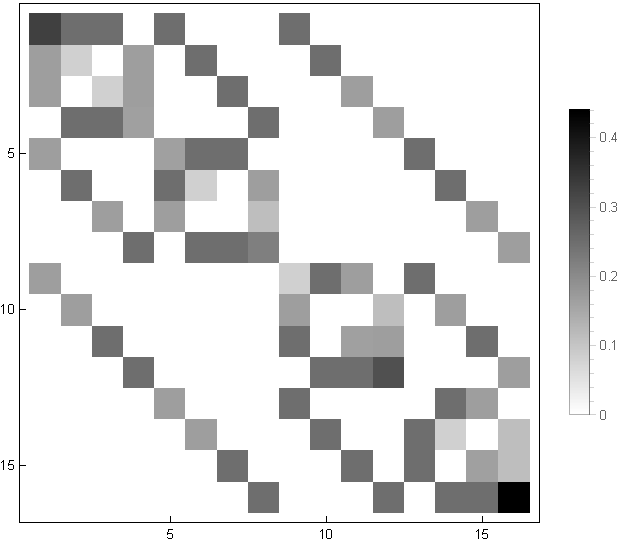
\includegraphics[width=0.23\linewidth]{../../NumCalc/ClassicalSpinStochMat/PROGRAMS/Mathematica/ArrayPlotM1_Beta0-1_Detailed.pdf}}
	\subcaptionbox{$\left\{\hat{M}_{[2,2]}(\beta)\right\}^{2}$\label{fig:fuga}}{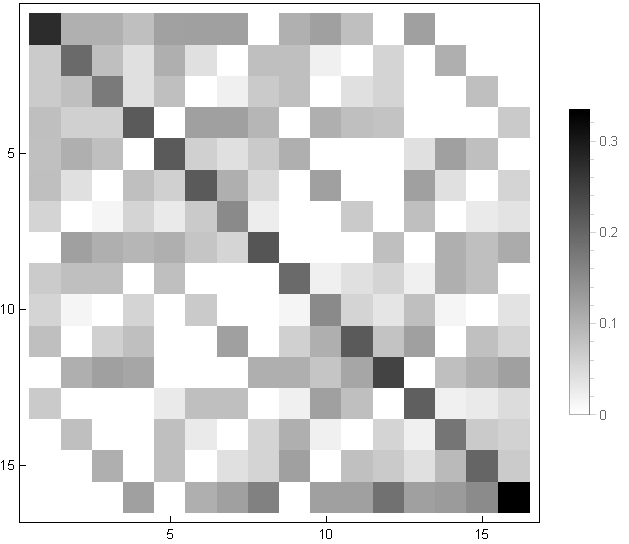
\includegraphics[width=0.23\linewidth]{../../NumCalc/ClassicalSpinStochMat/PROGRAMS/Mathematica/ArrayPlotM2_Beta0-1_Detailed.pdf}}
	\subcaptionbox{$\left\{\hat{M}_{[2,2]}(\beta)\right\}^{3}$\label{fig:fuga}}{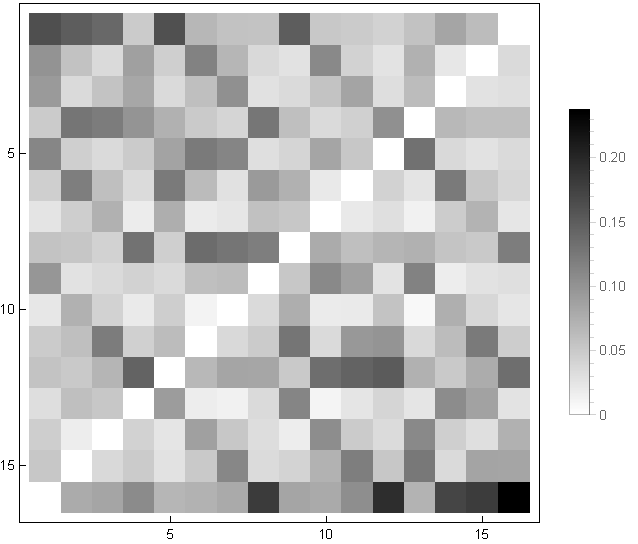
\includegraphics[width=0.23\linewidth]{../../NumCalc/ClassicalSpinStochMat/PROGRAMS/Mathematica/ArrayPlotM3_Beta0-1_Detailed.pdf}}
	\subcaptionbox{$\left\{\hat{M}_{[2,2]}(\beta)\right\}^{4}$\label{fig:fuga}}{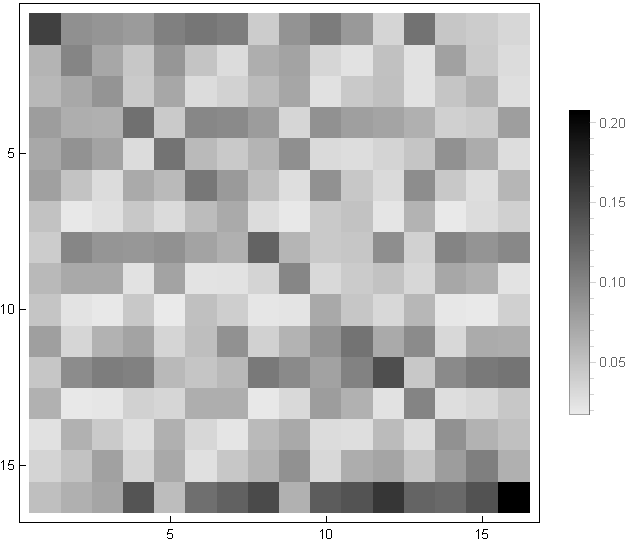
\includegraphics[width=0.23\linewidth]{../../NumCalc/ClassicalSpinStochMat/PROGRAMS/Mathematica/ArrayPlotM4_Beta0-1_Detailed.pdf}}
	\caption{The array plots of powers of $\hat{M}_{[2,2]}(\beta)$.}
\end{figure}

By the fact, we can see the existence of its unique stationary state as the long-time limit . In addition we investigated the distribution of the eigenvalues of $\hat{M}^{[2,2]}(\beta)$ for several temperatures and verified that the matrix $\hat{M}^{[2,2]}(\beta)$ has only an eigenvalue 1 and eigenvalue all inner than unit circle on the complex plane except for the case $\beta=0$ (See Figure \ref{fig:EigDistMbeta}).

\begin{figure}[htbp]
	\centering
	\subcaptionbox{$\beta=0$}{\includegraphics[width=0.3\linewidth]{../../NumCalc/ClassicalSpinStochMat/PROGRAMS/Mathematica/EigDist_M1_Beta0.pdf}}
	\subcaptionbox{$\beta=0.1$}{\includegraphics[width=0.3\linewidth]{../../NumCalc/ClassicalSpinStochMat/PROGRAMS/Mathematica/EigDist_M1_Beta0-1.pdf}}
	\subcaptionbox{$\beta=\infty$\label{fig:fuga}}{\includegraphics[width=0.3\linewidth]{../../NumCalc/ClassicalSpinStochMat/PROGRAMS/Mathematica/EigDist_M1_BetaInfinity.pdf}}
	\caption{The distributions of eigenvalues for $\hat{M}^{[2,2]}(\beta)$.}\label{fig:EigDistMbeta}
\end{figure}